\chapter{Your Central Work}

Lorem ipsum dolor sit amet, consectetuer adipiscing elit, sed diam nonummy nibh euismod tincidunt ut laoreet dolore magna aliquam erat volutpat. Ut wisi enim ad minim veniam, quis nostrud exerci tation ullamcorper suscipit lobortis nisl ut aliquip ex ea commodo consequat. Duis autem vel eum iriure dolor in hendrerit in vulputate velit esse molestie consequat, vel illum dolore eu feugiat nulla facilisis at vero et accumsan et iusto odio dignissim qui blandit.

\section{Variables}
The main thing we have to compute are particle positions. Accordingly, the most important variables for computing wind trajectories are the starting points and a velocity field. In our case, the starting points are defined by the user. The velocity field is extracted from a set of files containing assorted meteorological data.

For the most part, there are multiple files containing data at different points in time (10 minutes between files). Most of the actual data is stored in 3d arrays (plus some 2d ones for certain variables like surface height) whose axes correspond to rlon rlat level. Some of them are stored on a staggered grid, requiring interpolation if everything should be in the same coordinates.

Variables are: $U$ first velocity component (east-west), $V$ second velocity component (north-south), $W$ third velocity component (up-down), $lon$ and $lat$ coordinates in global system (or are those $\lambda$ and $\phi$?), $rlon$ and $rlat$ coordinates in rotated system, $level$ used in the $z$-axis of the grid, $h$ height above sea level (in meters) for the $z$-axis of actual positions, $HHL$ mapping levels to heights, $HSURF$ giving the surface height at  coordinates, $\delta t$ the size of our time step (in seconds), $t_{begin}$ and $t_{end}$ the start and end time of the simulation ... and that might be the interesting ones.

\section{Sampling}
\subsection{How LAGRANTO does it}
(TODO include pictures)

Sampling at $rlon$ $rlat$ $z$: The xy-coordinates of the 8 relevant grid points are easily computed from $rlon$ and $rlat$ (($rlon$-$rlon_min$)/$drlon$ etc). Each of the three axes has two associated weights. A local level-to-height map is built using a weighted sum of the nearby level heights. A binary search on this local level-to-height map gives the weights for the z-axis. The final value is then computed using simple trilinear interpolation.

\subsection{How I do it}
Same xy-weights, but replace the 2 fixed z-weights by separate ones for each corner. It is different.

\section{Method}
The tracing process starts by asking the user for initial points, start and end time, size of the timestep, and some optional parameters. After allocating space for the output data, the $UVW$ fields are extracted from the first three appropriate files. As the simulation runs, the oldest field is regularly replaced by new $UVW$ from the next file in line, minimizing the memory needed at runtime.
At each step, all trajectories have to be advanced by $\delta_t$. Those that have left the domain are kept at their last positions while the others get positions for the next timestep based on the velocity at their current position.

\subsection{Integrator}
LAGRANTO uses an iterative Euler scheme to compute $p_{t_0+\delta_t}$ from $p_{t_0}$ and $UVW(p, t)$:
\begin{equation}
	v_0 = UVW(p_{t_0}, t_0)
\end{equation}
\begin{equation}
	v_1 = UVW(p_{t_0}, t_0 + \delta_t)
\end{equation}
\begin{equation}
	q_1 = p_{t_0} + \delta_t \frac{ v_0  + v1}{2}
\end{equation}
\begin{equation}
	v_2 = UVW(q_1, t_0 + \delta_t)
\end{equation}
\begin{equation}
	q_2 = p_{t_0} + \delta_t \frac{ v_0  + v2}{2}
\end{equation}
\begin{equation}
	v_3 = UVW(q_2, t_0 + \delta_t)
\end{equation}
\begin{equation}
	p_{t_0 + \delta t} = p_{t_0} + \delta_t \frac{ v_0  + v3}{2}
\end{equation}
It works, but I still think it's not that good ... so Runge-Kutta
\begin{equation}
	k_1 = UVW(p_{t_0}, t_0)
\end{equation}
\begin{equation}
	k_1 = UVW(p_{t_0}, t_0)
\end{equation}
\begin{equation}
	k_1 = UVW(p_{t_0}, t_0)
\end{equation}
\begin{equation}
	k_1 = UVW(p_{t_0}, t_0)
\end{equation}

\section{Other sections}
To be put into other parts:

Lagranto description (earlier, Related Work), Results



\subsection{Fist Subsection}

Not sure if fist was a typo or on purpose, but it's funny

\subsection{Another Subsection}

\begin{table}
    \centering
    \begin{tabular}{|l|p{0.4\linewidth}|}
    \hline
    \emph{Quant.} & \emph{Ingredient}\\
    \hline
		200g &Wei{\ss}mehl\\
		1/4  &Packung Frischhefe\\
		4EL  &lauwarme Milch\\
		4EL  &�l\\
		1TL  &Zucker\\
		1TL  &Salz\\
		&lauwarmes Wasser\\
    \hline
    \end{tabular}
    \caption[Flammkuchenteig]{Flammkuchenteig. The ingredients have to be carefully chosen.\label{tab:mytable}}
\end{table}
\begin{figure}
    \centering
    \setlength{\tabcolsep}{0.0130\linewidth}
    \begin{tabular}{@{}cc@{}}
    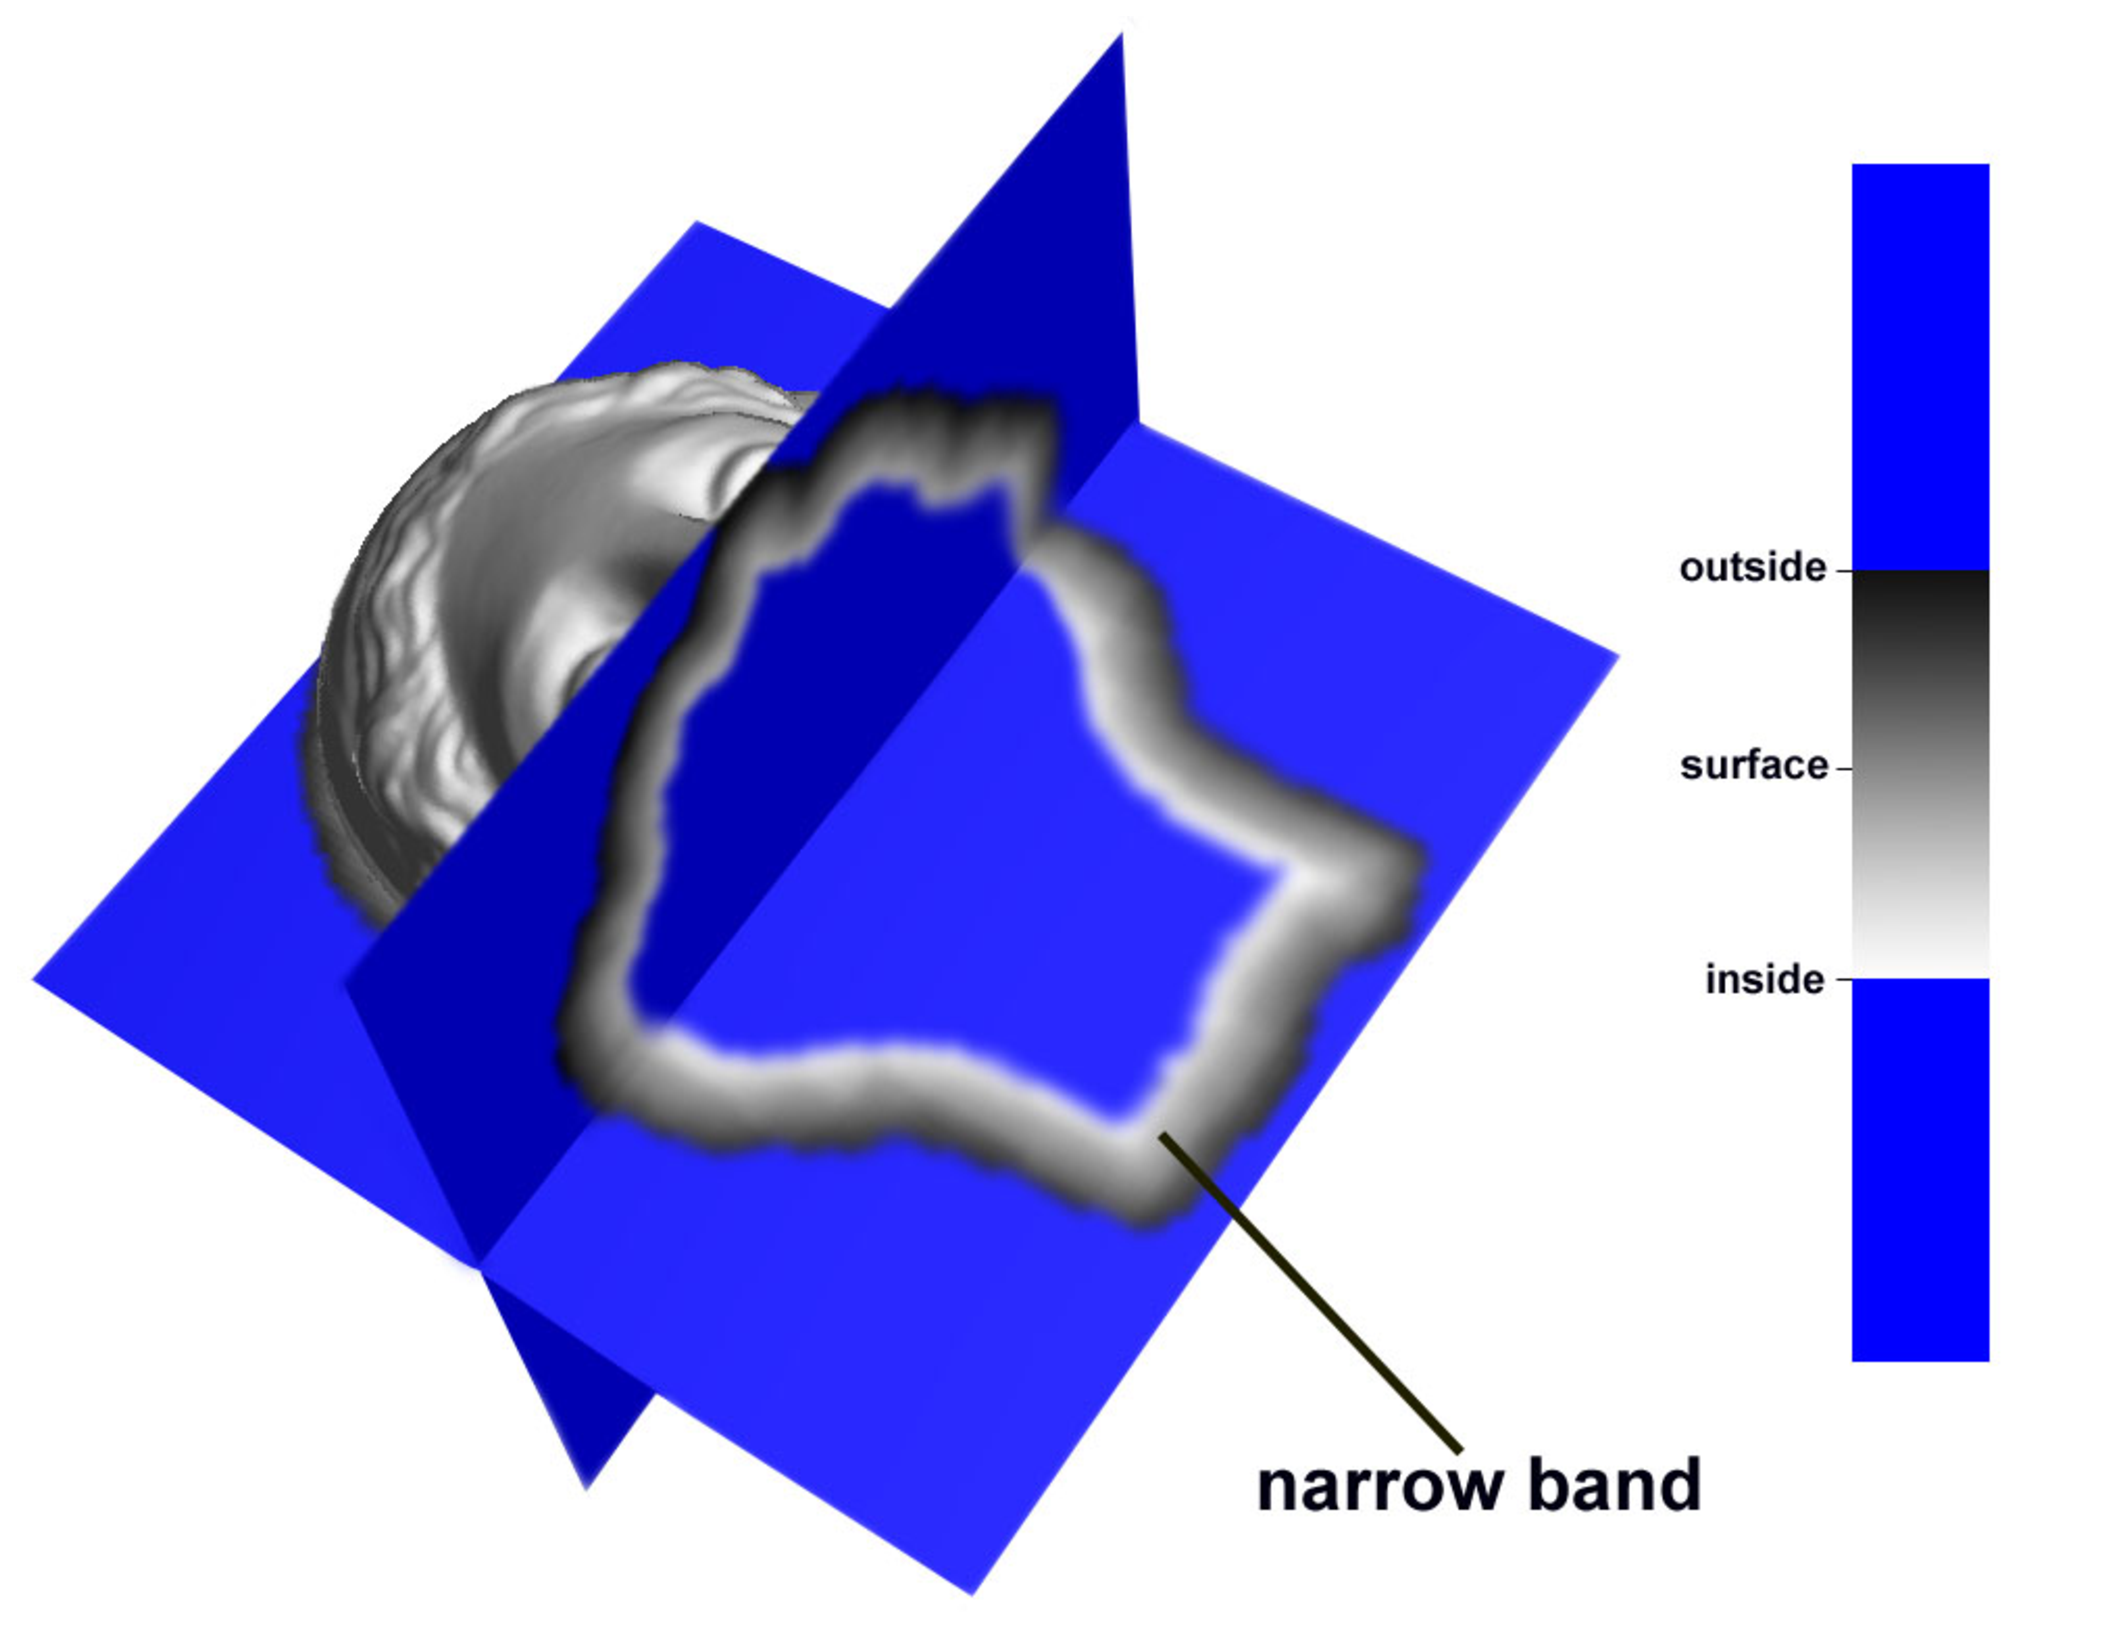
\includegraphics[width=0.487\linewidth]{figures/IgeaNarrowBand}&
    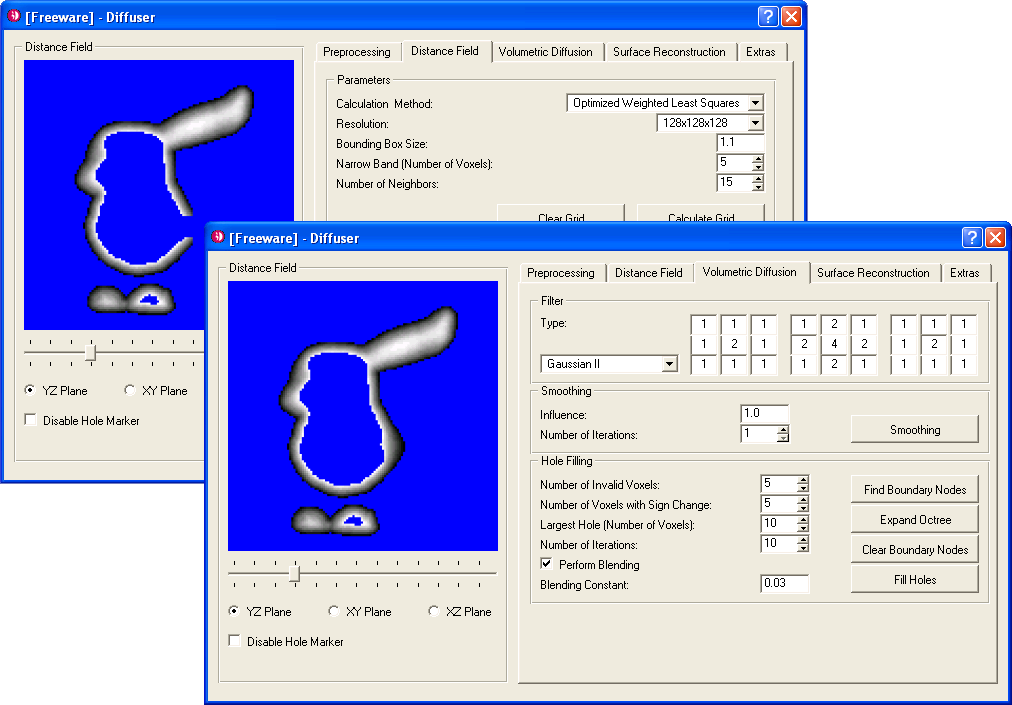
\includegraphics[width=0.487\linewidth]{figures/voldiff_ui}\\
    (a)&(b)\\
    \end{tabular}
    \caption[Volumetric diffusion]{Volumetric diffusion.
    	  \textup{(a)} Slices of the distance volume reveal the narrow band.
			  \textup{(b)} The user interface of the automatic hole filling
        tool allows to fine-tune the algorithm.
        The volumetric representation can be previewed before
        surface reconstruction.%
      \label{fig:voldiff}}
\end{figure}
\begin{figure}[!htb]
	\centering
	\subfigure[Caption first.]{\label{fig:test1}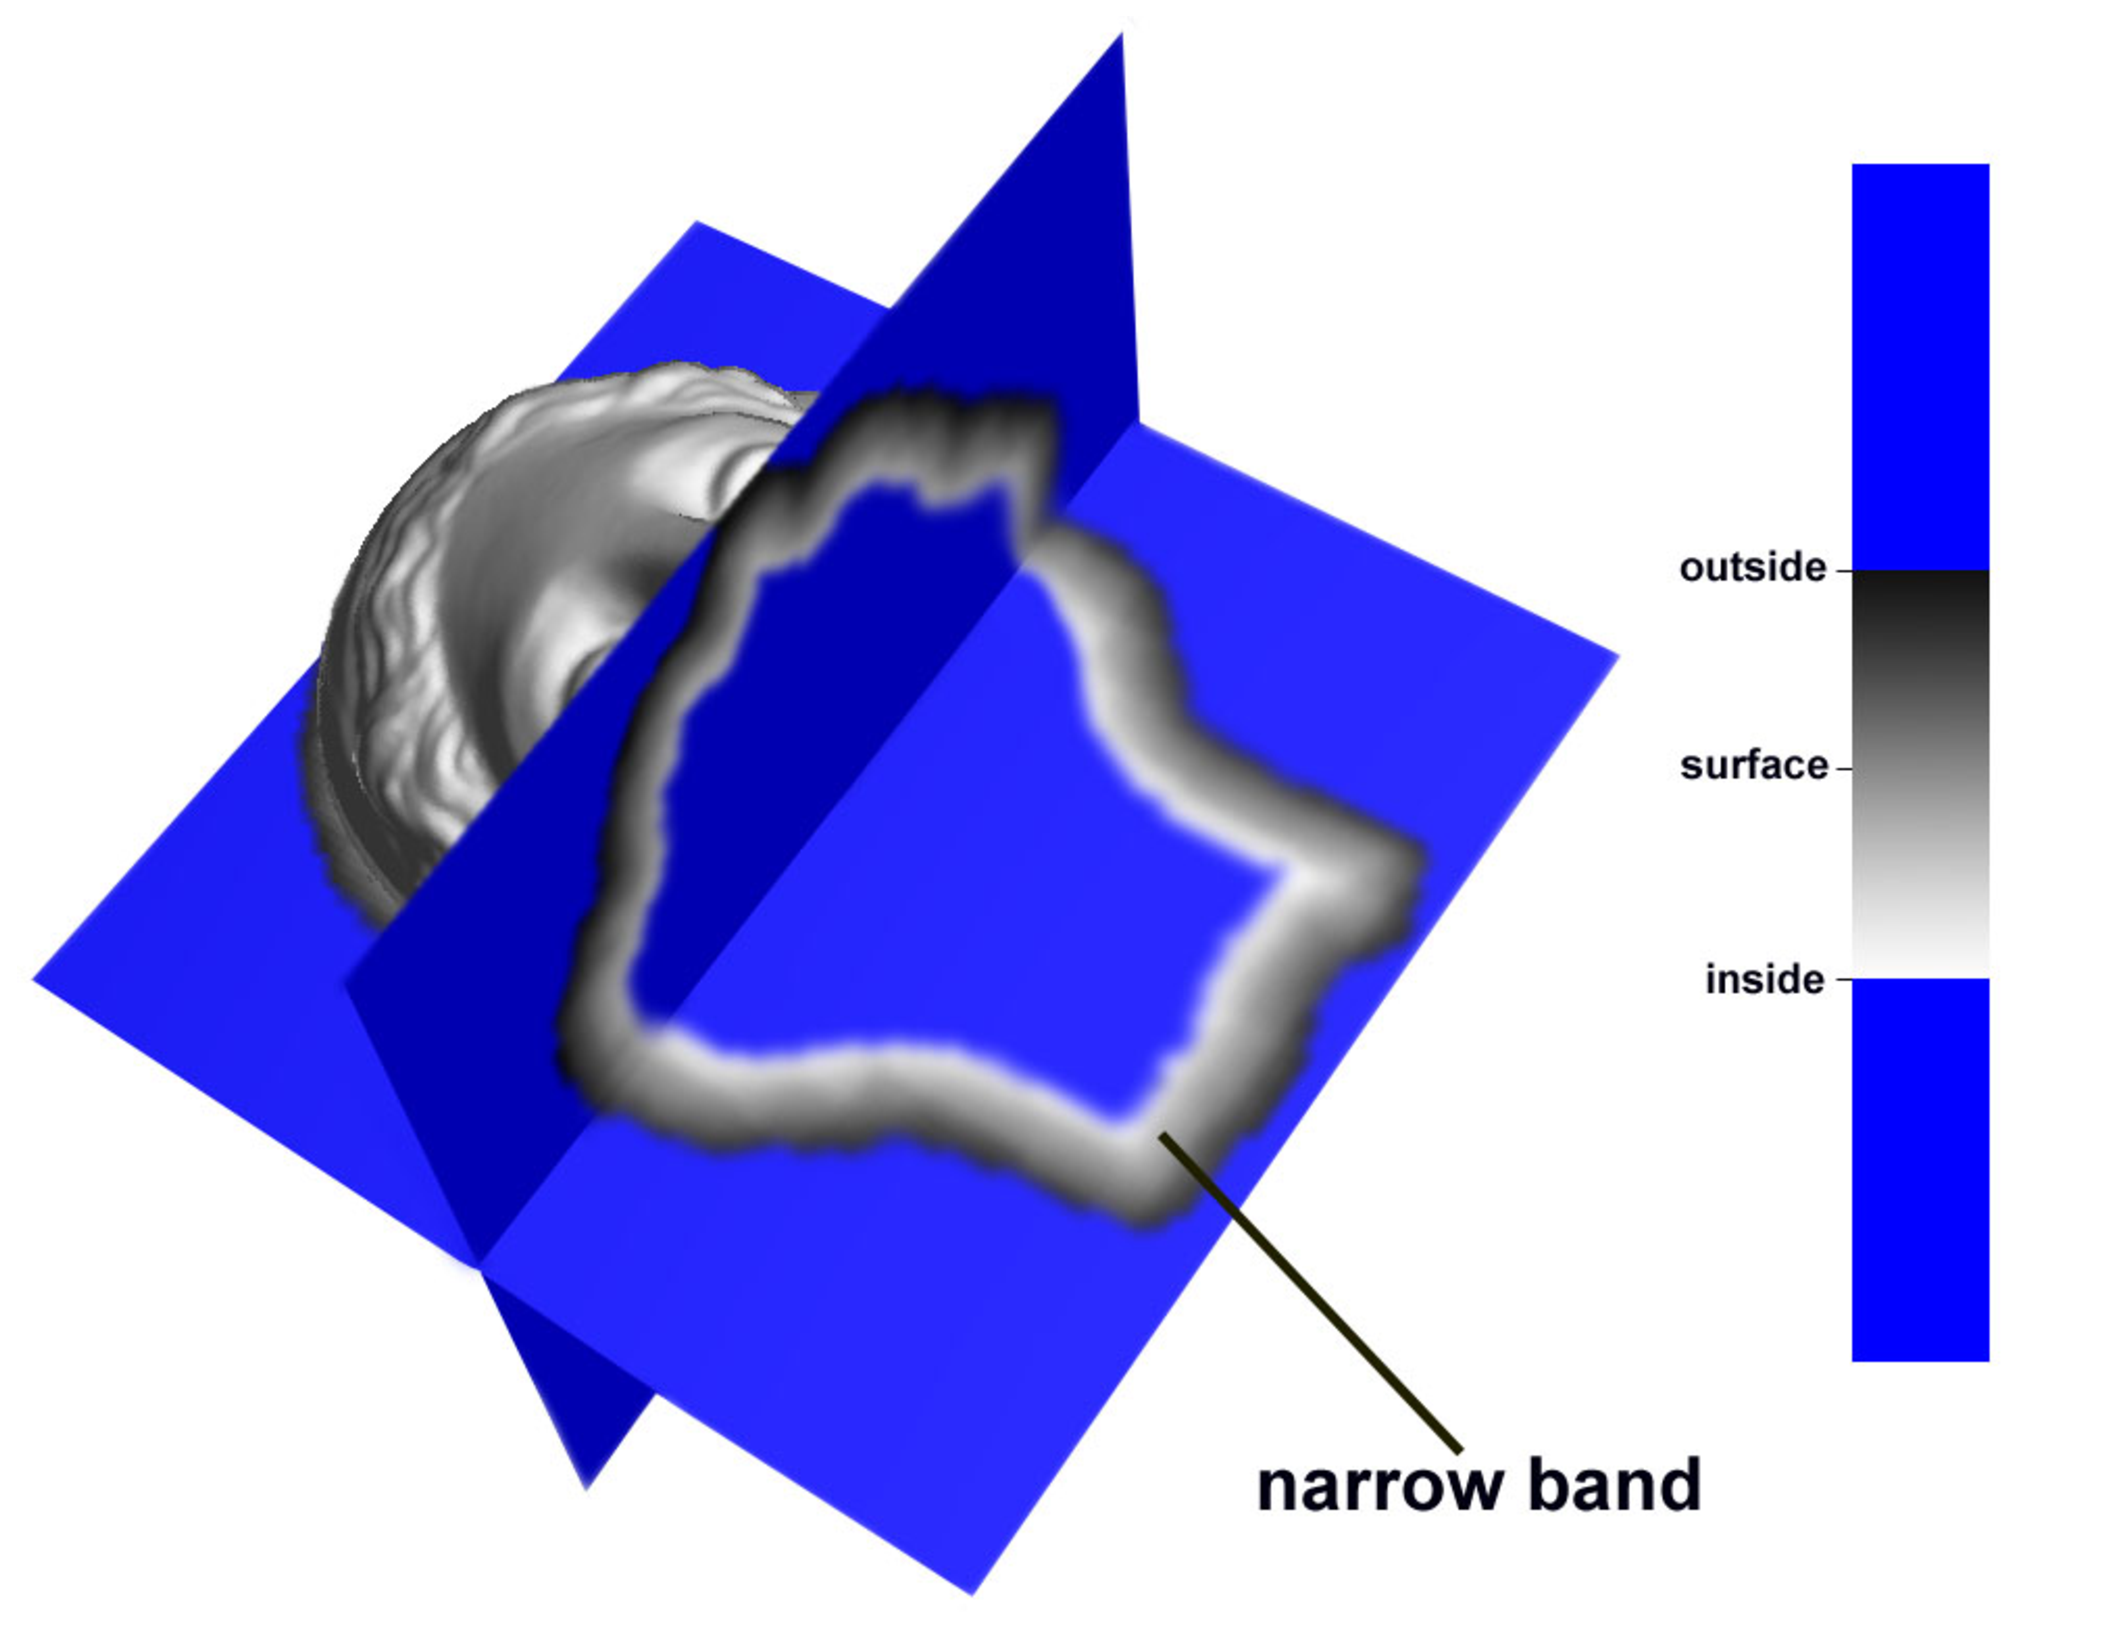
\includegraphics[width=0.3\textwidth]{figures/IgeaNarrowBand}} \hfill
	\subfigure[Caption second.]{\label{fig:test2}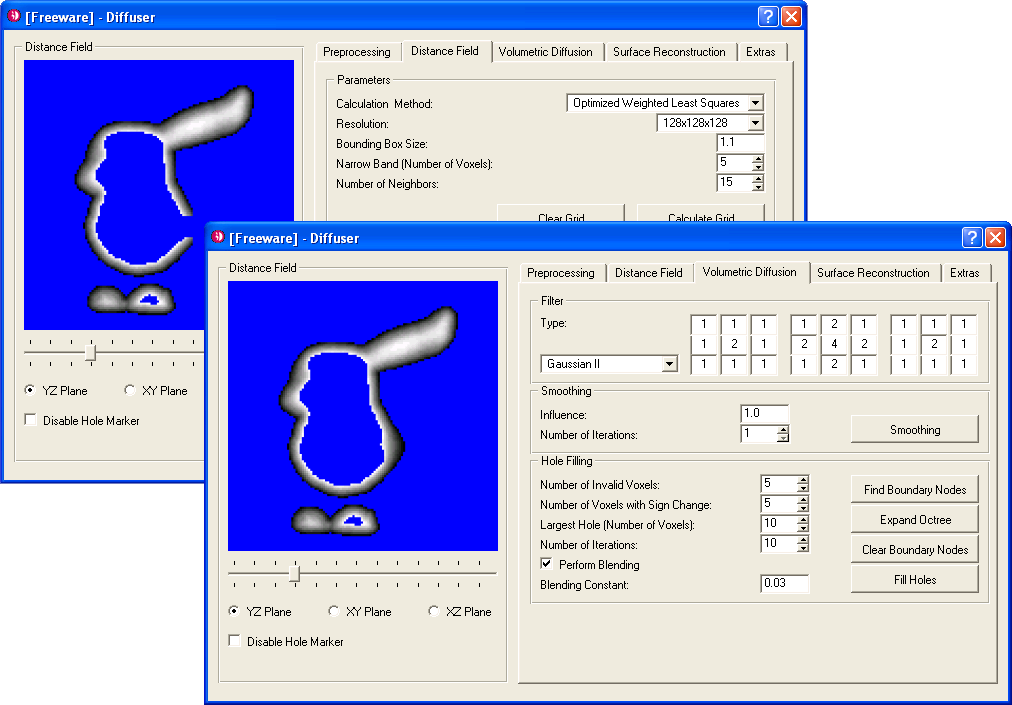
\includegraphics[width=0.3\textwidth]{figures/voldiff_ui}}
	\caption[Caption both]{Caption of both \subref{fig:test1}, \subref{fig:test2}.}
	\label{fig:bothfigures}
\end{figure}


Lorem ipsum dolor sit amet, consectetuer adipiscing elit, sed diam nonummy nibh euismod tincidunt ut laoreet dolore magna aliquam erat volutpat. Ut wisi enim ad minim veniam, quis nostrud exerci tation ullamcorper suscipit lobortis nisl ut aliquip ex ea commodo consequat. Duis autem vel eum iriure dolor in hendrerit in vulputate velit esse molestie consequat, vel illum dolore eu feugiat nulla facilisis at vero et accumsan et iusto odio dignissim qui blandit praesent luptatum zzril delenit augue duis dolore te feugait nulla facilisi. Lorem ipsum dolor sit amet, consectetuer adipiscing elit, sed diam 

\section{Second Section}

That's not really the second section!
